\documentclass{article}
%%%%%%%%%%%%%%%%%%%%%%%%%%%%%%%%%%%%%%%%%%%%%%%%%%%%%%%%%%%%%
% Lecture Specific Information to Fill Out
%%%%%%%%%%%%%%%%%%%%%%%%%%%%%%%%%%%%%%%%%%%%%%%%%%%%%%%%%%%%%
\newcommand{\LectureTitle}{Lectures Week \#1 Notes}
%\newcommand{\LectureDate}{\today}
\newcommand{\LectureDate}{July\ 30,\ 2013}
\newcommand{\LectureClassName}{MATH\ 3511}
\newcommand{\LatexerName}{Professor\ James\ Franklin}
%%%%%%%%%%%%%%%%%%%%%%%%%%%%%%%%%%%%%%%%%%%%%%%%%%%%%%%%%%%%%

% Change "article" to "report" to get rid of page number on title page
\usepackage{amsmath,amsfonts,amsthm,amssymb}
\usepackage{setspace}
\usepackage{Tabbing}
\usepackage{fancyhdr}
\usepackage{lastpage}
\usepackage{extramarks}
\usepackage{chngpage}
\usepackage{soul,color}
\usepackage{graphicx,float,wrapfig}
\usepackage{afterpage}
\usepackage{abstract}

\usepackage[parfill]{parskip}
% recommended from http://poisson.phc.unipi.it/~maggiolo/index.php/2008/12/latex-class-for-lecture-notes/
\usepackage[pdf]{pstricks}
\usepackage{pst-plot}
\usepackage{hyperref}
\usepackage{mathtools}
\usepackage{booktabs}
\usepackage{multirow}
\usepackage{fancyhdr}
\usepackage{mparhack}
\usepackage{tikz}
\usepackage{mathdots}
\usepackage{xfrac}
\usepackage{faktor}
\usepackage{cancel}

% In case you need to adjust margins:
\topmargin=-0.45in
\evensidemargin=0in
\oddsidemargin=0in
\textwidth=6.5in
\textheight=9.0in
\headsep=0.25in

% Setup the header and footer
\pagestyle{fancy}
\lhead{\LatexerName}
\chead{\LectureClassName: \LectureTitle}
\rhead{\LectureDate}
\lfoot{\lastxmark}
\cfoot{}
\rfoot{Page\ \thepage\ of\ \pageref{LastPage}}
\renewcommand\headrulewidth{0.4pt}
\renewcommand\footrulewidth{0.4pt}

%%%%%%%%%%%%%%%%%%%%%%%%%%%%%%%%%%%%%%%%%%%%%%%%%%%%%%%%%%%%%
% Some tools
\newcommand{\enterTopicHeader}[1]{\nobreak\extramarks{#1}{#1 continued on next page\ldots}\nobreak
                                    \nobreak\extramarks{#1 (continued)}{#1 continued on next page\ldots}\nobreak}
\newcommand{\exitTopicHeader}[1]{\nobreak\extramarks{#1 (continued)}{#1 continued on next page\ldots}\nobreak
                                   \nobreak\extramarks{#1}{}\nobreak}

\newlength{\labelLength}
\newcommand{\labelAnswer}[2]
  {\settowidth{\labelLength}{#1}
   \addtolength{\labelLength}{0.25in}
   \changetext{}{-\labelLength}{}{}{}
   \noindent\fbox{\begin{minipage}[c]{\columnwidth}#2\end{minipage}}
   \marginpar{\fbox{#1}}

   % We put the blank space above in order to make sure this
   % \marginpar gets correctly placed.
   \changetext{}{+\labelLength}{}{}{}}

\setcounter{secnumdepth}{0}
\newcommand{\TopicName}{}
\newcounter{TopicCounter}
\newenvironment{Topic}[1][Problem \arabic{TopicCounter}]
  {\stepcounter{TopicCounter}
   \renewcommand{\TopicName}{#1}
   \section{\TopicName}
   \enterTopicHeader{\TopicName}}
  {\exitTopicHeader{\TopicName}}
  
\setcounter{secnumdepth}{0}
\newcommand{\ExampleSectionName}{}
\newcounter{ExampleSectionCounter}[TopicCounter]
\newenvironment{ExampleSection}[1][Example \arabic{ExampleSectionCounter}]
  {\stepcounter{ExampleSectionCounter}
   \renewcommand{\ExampleSectionName}{#1}
   \section{\ExampleSectionName}
   \enterTopicHeader{\ExampleSectionName}}
  {\exitTopicHeader{\ExampleSectionName}}

\setcounter{secnumdepth}{0}
\newcounter{ExampleBoxCounter}[TopicCounter]
\newcommand{\examplebox}[1]
  {
  % We put this space here to make sure we're disconnected from the previous
   % passage
   \stepcounter{ExampleBoxCounter}
   \noindent\fbox{\begin{minipage}[c]{\columnwidth}#1\end{minipage}}\enterTopicHeader{\ExampleSectionName}\exitTopicHeader{\ExampleSectionName}\marginpar{\fbox{\#\arabic{ExampleBoxCounter}}}
   % We put the blank space above in order to make sure this
   % \marginpar gets correctly placed.
   \vskip10pt
   }

\renewcommand{\contentsname}{{\normalsize Topics Covered}}
\renewcommand{\abstractname}{\LectureTitle\ Summary}
\renewcommand{\absnamepos}{flushleft}

%%%%%%%%%%%%%%%%%%%%%%%%%%%%%%%%%%%%%%%%%%%%%%%%%%%%%%%%%%%%%

\begin{document}
\begin{spacing}{1.1}
\newpage

\begin{abstract}
Prepared by Laurence Davies
\end{abstract}

\tableofcontents
\addtocontents{toc}{~\hfill\textbf{Page}\par}
\vskip10pt
\hrule
\vskip10pt

% When topics are long, it may be desirable to put a \newpage or a
% \clearpage before each Topic environment
%\newpage
\begin{Topic}[\Roman{TopicCounter} Introduction]
There are three main parts to this course:

\begin{enumerate}
\item Geometry (extra Euclidean geometry)
  \begin{itemize}
    \item Centres of triangles (mean, circumcentre, and so on)
    \item Circles
  \end{itemize}
\item Transformations in geometry 
  \begin{itemize}
    \item (Rotations, reflections, glide reflections, similarities) 
  \end{itemize}
\item Groups (abstract algebra) 
  \begin{itemize}
    \item e.g. Groups of symmetries:\\
%          \examplebox{

Consider the reflective symmetries of an equilateral triangle.\\ \\
% Generated with LaTeXDraw 2.0.8
% Tue Jul 30 12:28:22 EST 2013
% \usepackage[usenames,dvipsnames]{pstricks}
% \usepackage{epsfig}
% \usepackage{pst-grad} % For gradients
% \usepackage{pst-plot} % For axes
\begin{center}
\scalebox{0.7} % Change this value to rescale the drawing.
{
\begin{pspicture}(0,-3.69)(10.03,3.79)
\pstriangle[linewidth=0.04,dimen=outer](5.42,-1.39)(5.08,3.98)
\psline[linewidth=0.04cm,linestyle=dashed,dash=0.16cm 0.16cm](8.98,-1.95)(2.82,1.47)
\psline[linewidth=0.04cm,linestyle=dashed,dash=0.16cm 0.16cm](2.0,-1.83)(7.88,1.35)
\psline[linewidth=0.04cm,linestyle=dashed,dash=0.16cm 0.16cm](5.44,-2.57)(5.42,3.77)
\psdots[dotsize=0.12](5.46,0.01)
\psarc[linewidth=0.04,arrowsize=0.05291667cm 2.0,arrowlength=1.4,arrowinset=0.4]{<-}(8.91,-1.92){0.35}{58.24052}{217.40535}
\psarc[linewidth=0.04,arrowsize=0.05291667cm 2.0,arrowlength=1.4,arrowinset=0.4]{<-}(2.33,-1.68){0.35}{304.11447}{117.474434}
\psarc[linewidth=0.04,arrowsize=0.05291667cm 2.0,arrowlength=1.4,arrowinset=0.4]{<-}(5.43,3.02){0.35}{357.27368}{182.48955}
\usefont{T1}{ptm}{m}{n}
\rput(7.76,-3.085){Reflective symmetries}
\pscustom[linewidth=0.01]
{
\newpath
\moveto(9.26,-2.85)
\lineto(9.28,-2.8)
\curveto(9.29,-2.775)(9.305,-2.705)(9.31,-2.66)
\curveto(9.315,-2.615)(9.32,-2.53)(9.32,-2.49)
\curveto(9.32,-2.45)(9.3,-2.375)(9.28,-2.34)
\curveto(9.26,-2.305)(9.22,-2.255)(9.2,-2.24)
\curveto(9.18,-2.225)(9.14,-2.205)(9.08,-2.19)
}
\pscustom[linewidth=0.01]
{
\newpath
\moveto(9.34,-2.85)
\lineto(9.47,-2.65)
\curveto(9.535,-2.55)(9.715,-2.25)(9.83,-2.05)
\curveto(9.945,-1.85)(10.025,-1.575)(9.99,-1.5)
\curveto(9.955,-1.425)(9.9,-1.305)(9.88,-1.26)
\curveto(9.86,-1.215)(9.825,-1.13)(9.81,-1.09)
\curveto(9.795,-1.05)(9.615,-0.73)(9.45,-0.45)
\curveto(9.285,-0.17)(8.975,0.32)(8.83,0.53)
\curveto(8.685,0.74)(8.51,1.025)(8.48,1.1)
\curveto(8.45,1.175)(8.33,1.435)(8.24,1.62)
\curveto(8.15,1.805)(8.005,2.03)(7.95,2.07)
\curveto(7.895,2.11)(7.6,2.28)(7.36,2.41)
\curveto(7.12,2.54)(6.765,2.715)(6.65,2.76)
\curveto(6.535,2.805)(6.385,2.855)(6.35,2.86)
\curveto(6.315,2.865)(6.265,2.89)(6.25,2.91)
\curveto(6.235,2.93)(6.21,2.95)(6.18,2.95)
}
\pscustom[linewidth=0.01]
{
\newpath
\moveto(9.42,-3.13)
\lineto(9.44,-3.16)
\curveto(9.45,-3.175)(9.46,-3.23)(9.46,-3.27)
\curveto(9.46,-3.31)(9.405,-3.38)(9.35,-3.41)
\curveto(9.295,-3.44)(9.17,-3.49)(9.1,-3.51)
\curveto(9.03,-3.53)(8.725,-3.55)(8.49,-3.55)
\curveto(8.255,-3.55)(7.92,-3.56)(7.82,-3.57)
\curveto(7.72,-3.58)(7.225,-3.61)(6.83,-3.63)
\curveto(6.435,-3.65)(5.9,-3.675)(5.76,-3.68)
\curveto(5.62,-3.685)(5.015,-3.655)(4.55,-3.62)
\curveto(4.085,-3.585)(3.52,-3.475)(3.42,-3.4)
\curveto(3.32,-3.325)(3.12,-3.155)(3.02,-3.06)
\curveto(2.92,-2.965)(2.8,-2.835)(2.78,-2.8)
\curveto(2.76,-2.765)(2.725,-2.68)(2.71,-2.63)
\curveto(2.695,-2.58)(2.67,-2.505)(2.66,-2.48)
\curveto(2.65,-2.455)(2.635,-2.405)(2.63,-2.38)
\curveto(2.625,-2.355)(2.62,-2.305)(2.62,-2.28)
\curveto(2.62,-2.255)(2.62,-2.205)(2.62,-2.18)
\curveto(2.62,-2.155)(2.62,-2.115)(2.62,-2.07)
}
\psarc[linewidth=0.04,arrowsize=0.05291667cm 2.0,arrowlength=1.4,arrowinset=0.4]{<-}(5.18,0.03){2.68}{94.87927}{200.6589}
\psarc[linewidth=0.04,arrowsize=0.05291667cm 2.0,arrowlength=1.4,arrowinset=0.4]{<-}(5.39,0.0){3.77}{338.8539}{200.0}
\usefont{T1}{ptm}{m}{n}
\rput(2.99,0.195){120}
\usefont{T1}{ptm}{m}{n}
\rput(1.71,1.875){240}
\usefont{T1}{ptm}{m}{n}
\rput(1.63,3.595){Rotational symmetries}
\end{pspicture} 
}
\end{center}



%}
    \item There will also be material on freeze groups and wallpaper groups.
  \end{itemize}
\end{enumerate}
\end{Topic}

\begin{Topic}[\Roman{TopicCounter} Historical Example: Lunes]
The following considers an ancient text on Hippocrates Lunes (\textasciitilde450BC).

\begin{figure*}[t]
\centering
\scalebox{1} % Change this value to rescale the drawing.
{
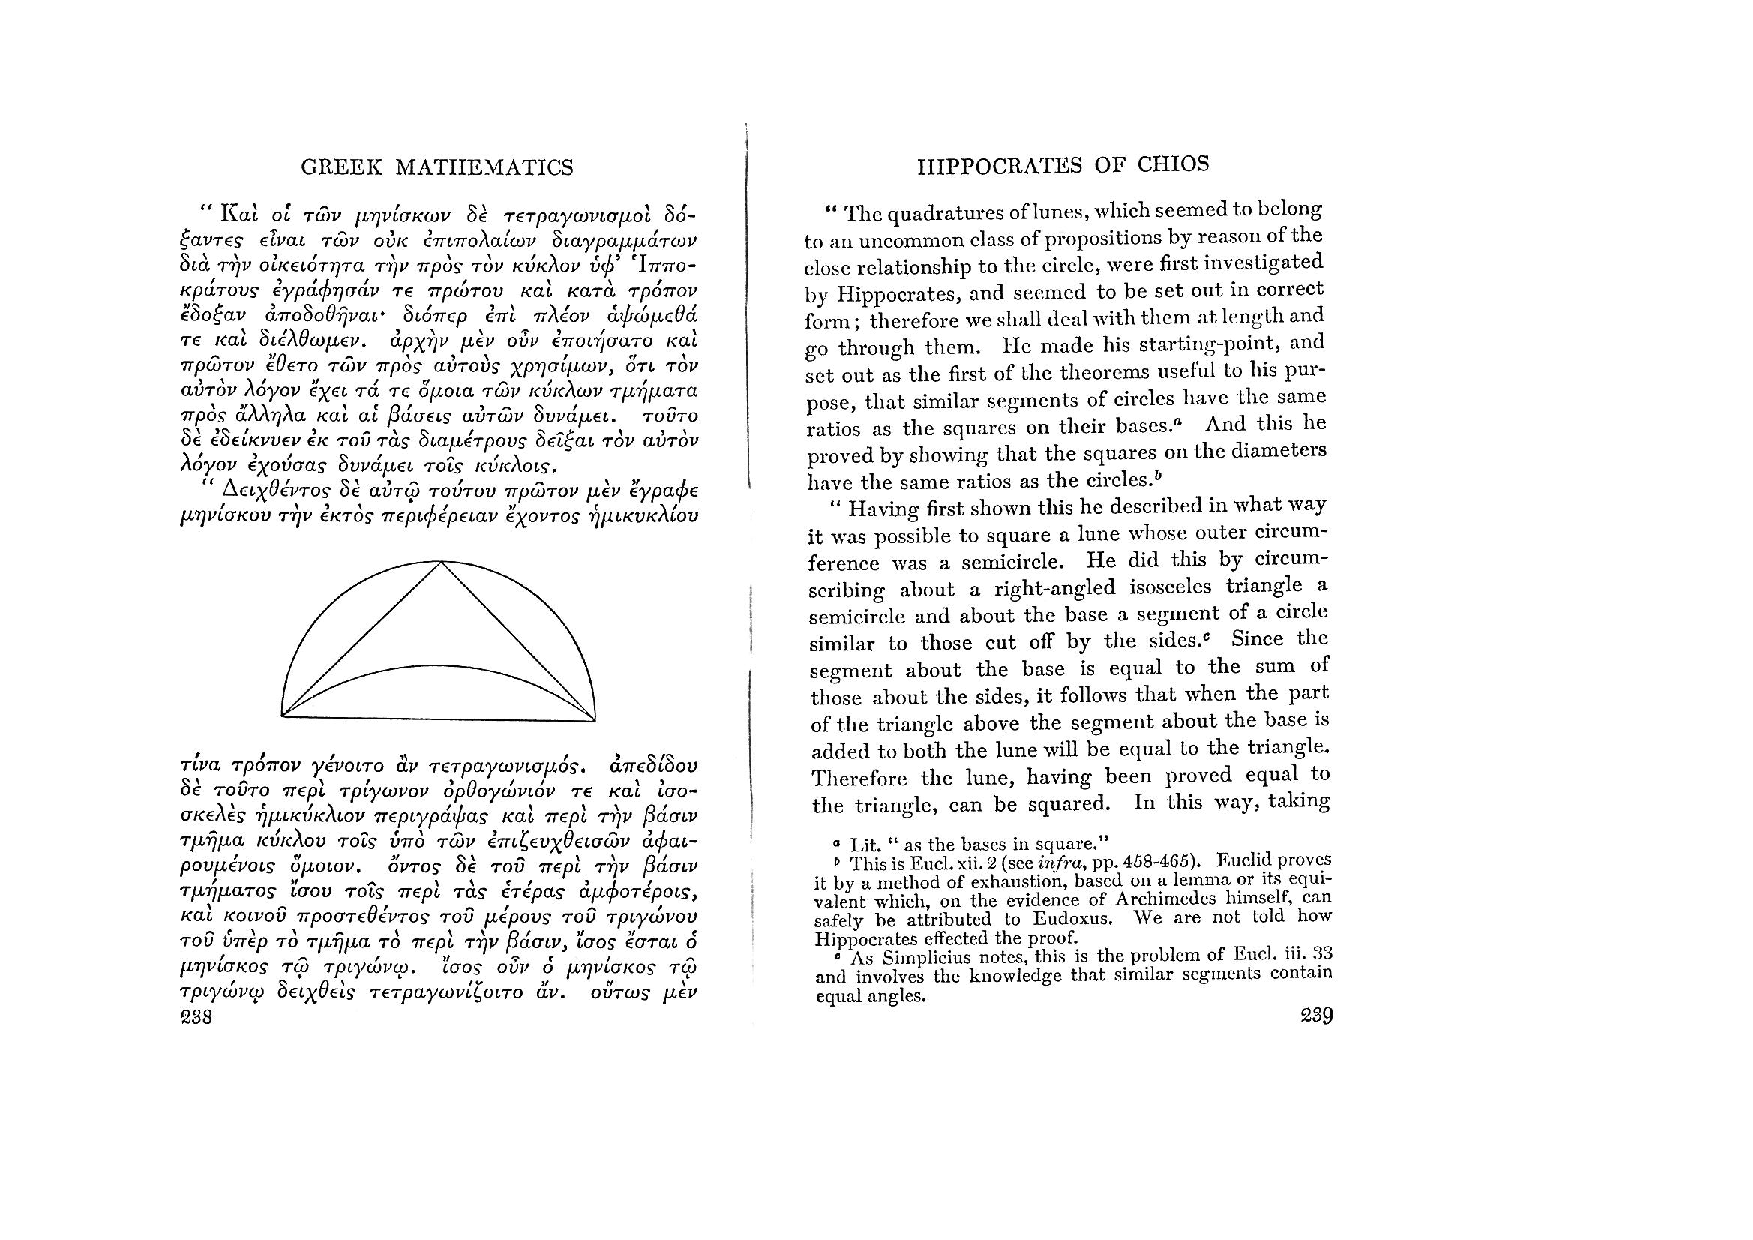
\includegraphics[width=1.0\textwidth]{Figures/hippocrateslunes_crop.pdf}
}
%\caption{From <reference>}
\end{figure*}

%\begin{ExampleSection}
Find a square with the same area as a curved lune.\\

% Generated with LaTeXDraw 2.0.8
% Tue Jul 30 12:48:41 EST 2013
% \usepackage[usenames,dvipsnames]{pstricks}
% \usepackage{epsfig}
% \usepackage{pst-grad} % For gradients
% \usepackage{pst-plot} % For axes
\begin{center}
\scalebox{1} % Change this value to rescale the drawing.
{
\begin{pspicture}(0,4.2331495)(14.4952,10.2876005)
\pswedge[linewidth=0.04](8.475201,4.2676){6.0}{0.0}{180.0}
\pstriangle[linewidth=0.04,dimen=outer](8.475201,4.2576003)(12.0,6.0)
\psarc[linewidth=0.04](8.4852,-1.7823999){8.4852}{45.558964}{134.65895}
\psline[linewidth=0.04](14.426324,4.27579)(2.5210772,4.2531495)
\usefont{T1}{ptm}{m}{n}
\rput(8.4852,5.7226){C}
\usefont{T1}{ptm}{m}{n}
\rput(5.4752,8.3226){A}
\usefont{T1}{ptm}{m}{n}
\rput(11.5452,8.3426){B}
\usefont{T1}{ptm}{m}{n}
\rput(8.4552,8.1826){D}
\rput{-45.0}(-4.569971,8.922314){\psframe[linewidth=0.04,dimen=outer](8.6852,10.1776)(8.2852,9.7776)}
\usefont{T1}{ptm}{m}{n}
\rput(6.2252,7.7426){a}
\usefont{T1}{ptm}{m}{n}
\rput(10.5852,7.7626){b}
\usefont{T1}{ptm}{m}{n}
\rput(8.4652,4.5026){c}
\end{pspicture} 
}
\end{center}


Examine areas $A$, $B$, $C$ and $D$. This example will show that $C=A+B$ and hence the area of the lune $A+D+B=C+D$ which is the area of the triangle $\frac{1}{2}\times base\times height$.\\

Consider the Pythagorean relationship $c^2=a^2+b^2$.\\

The relationship between an area and the corresponding chord length is a quadrature 
i.e. $A = \lambda a^2$ where $\lambda$ is the same for all three segments.


%\end{ExampleSection}
\end{Topic}



\newpage


\begin{Topic}[\Roman{TopicCounter} Euclid's Elements]

As a brief introduction to Euclids Elements, this section will discuss one or two items from the definitions, postulates, common notions and propositions\footnote{For a more comprehensive list of definitions, postulates and common notions, see \textit{http://aleph0.clarku.edu/\textasciitilde djoyce/java/elements/elements.html}}.

In proposition 1\footnote{\\\textit{http://aleph0.clarku.edu/~djoyce/java/elements/bookI/propI1.html}}
\textbf{"To construct an equilateral triangle on a given finite straight line"} there are areas that
can be subject to critique, such as the notion that the circles must intersect. Without this intersection,
C cannot be described and thus the proposition does not hold, but Euclid does not explicitly explain how they
must intersect. This aspect as well as others are the subject of deeper mathematics that was explored by
Hilbert and G\"{o}del (in his Incompleteness Theorems).

Aristotle (who predated Euclid) proposed that every science be organised as a set of propositions 
deduced from \textit{self-evident} axioms, definitions and postulates. If it is organised in such a way,
everything that follows is certain and there would be no need for measurement or observation.

Unfortunately, this did not work for most sciences but it did work for mathematics, in particular in number theory.

There are two common definitions of geometry. The first is pure (Euclidean) geometry, and the second is the shape of space (as explored in physics). This course aims to focus on the first.

Consider the preliminary example of two triangles described by two lines intersecting between two parallel lines as below.

% Generated with LaTeXDraw 2.0.8
% Thu Aug 01 13:09:25 EST 2013
% \usepackage[usenames,dvipsnames]{pstricks}
% \usepackage{epsfig}
% \usepackage{pst-grad} % For gradients
% \usepackage{pst-plot} % For axes
\begin{center}
\scalebox{1} % Change this value to rescale the drawing.
{
\begin{pspicture}(0,-2.0)(3.4803584,2.0)
\psline[linewidth=0.04cm,arrowsize=0.05291667cm 2.0,arrowlength=1.4,arrowinset=0.4]{<-}(0.0,1.14)(3.4603584,1.14)
\psline[linewidth=0.04cm,arrowsize=0.05291667cm 2.0,arrowlength=1.4,arrowinset=0.4]{<-}(0.0,-1.54)(3.4603584,-1.54)
\psline[linewidth=0.04cm](0.9002299,1.92)(2.70023,-1.94)
\psline[linewidth=0.04cm](0.22022985,-1.98)(2.7402298,1.98)
\usefont{T1}{ptm}{m}{n}
\rput(1.5002298,0.965){a}
\usefont{T1}{ptm}{m}{n}
\rput(0.86022985,-1.355){a}
\usefont{T1}{ptm}{m}{n}
\rput(1.9002298,0.945){b}
\usefont{T1}{ptm}{m}{n}
\rput(2.12023,-1.355){b}
\usefont{T1}{ptm}{m}{n}
\rput(1.6602298,-0.095){c}
\usefont{T1}{ptm}{m}{n}
\rput(1.6802299,0.585){c}
\end{pspicture} 
}
\end{center}


These triangles can be said to be similar because it can be shown that the corresponding angles are equal. The corresponding angle pairs $a$ and $b$ are alternate angles in parallel lines, and the angle pair $c$ are simply opposite angles described by intersecting straight lines. It can be then stated that these similar triangles have corresponding sides in the same ratio.\\

\textbf{Geometry of Circles}\\

Consider the figure below which describes the angles at the centre and circumference of a circle described by a chord.

% Generated with LaTeXDraw 2.0.8
% Thu Aug 01 13:19:56 EST 2013
% \usepackage[usenames,dvipsnames]{pstricks}
% \usepackage{epsfig}
% \usepackage{pst-grad} % For gradients
% \usepackage{pst-plot} % For axes
\begin{center}
\scalebox{1} % Change this value to rescale the drawing.
{
\begin{pspicture}(0,-2.91)(5.42,2.51)
\pscircle[linewidth=0.04,dimen=outer](2.71,-0.2){2.71}
\psdots[dotsize=0.12](2.72,-0.17)
\psline[linewidth=0.04](2.7,-0.15)(1.38,-2.41)(2.6,2.47)(5.22,-1.09)(2.72,-0.15)
\psarc[linewidth=0.04](2.62,2.47){0.44}{254.74489}{302.4712}
\psarc[linewidth=0.04,linestyle=dashed,dash=0.16cm 0.16cm](2.61,0.2){0.81}{258.02386}{316.6847}
\psline[linewidth=0.04cm,linestyle=dashed,dash=0.16cm 0.16cm](1.38,-2.51)(5.22,-1.11)
\usefont{T1}{ptm}{m}{n}
\rput(3.4,-2.065){chord}
\usefont{T1}{ptm}{m}{n}
\rput(2.93,0.035){0}
\end{pspicture} 
}
\end{center}



It is required to prove that \textbf{the angle at the centre is twice the angle at the circumference subtended by the same chord}.

\begin{enumerate}
\item Construct a line from the vertex of the angle on the circumference passing through the centre of the circle.
\item The segment of the line from the vertex to the centre is the radius, and thus forms two isosceles triangles as depicted below
% Generated with LaTeXDraw 2.0.8
% Thu Aug 01 13:45:24 EST 2013
% \usepackage[usenames,dvipsnames]{pstricks}
% \usepackage{epsfig}
% \usepackage{pst-grad} % For gradients
% \usepackage{pst-plot} % For axes
\begin{center}
\scalebox{1} % Change this value to rescale the drawing.
{
\begin{pspicture}(0,-2.71)(5.42,2.71)
\pscircle[linewidth=0.04,dimen=outer](2.71,0.0){2.71}
\psdots[dotsize=0.12](2.72,0.03)
\psline[linewidth=0.04](2.7,0.05)(1.38,-2.21)(2.6,2.67)(5.22,-0.89)(2.72,0.05)
\usefont{T1}{ptm}{m}{n}
\rput(2.99,0.155){0}
\psline[linewidth=0.04cm](2.76,-1.37)(2.62,2.63)
\psline[linewidth=0.04cm,linestyle=dashed,dash=0.16cm 0.16cm](2.08,-0.87)(2.22,-0.99)
\psline[linewidth=0.04cm,linestyle=dashed,dash=0.16cm 0.16cm](3.84,-0.27)(3.8,-0.45)
\psline[linewidth=0.04cm,linestyle=dashed,dash=0.16cm 0.16cm](2.62,1.11)(2.76,1.11)
\usefont{T1}{ptm}{m}{n}
\rput(2.53,1.835){x}
\usefont{T1}{ptm}{m}{n}
\rput(2.89,1.995){y}
\usefont{T1}{ptm}{m}{n}
\rput(1.79,-1.105){x}
\usefont{T1}{ptm}{m}{n}
\rput(4.35,-0.165){y}
\usefont{T1}{ptm}{m}{n}
\rput(2.52,-0.805){2x}
\usefont{T1}{ptm}{m}{n}
\rput(3.1,-0.545){2y}
\end{pspicture} 
}
\end{center}

\item The exterior angle of a triangle is the sum of the opposing two interior angles (shown later). Thus the angle at the centre is $2x + 2y$, which is twice the angle at the circumference $x + y$.
\end{enumerate}

Two corollaries can be derived from this proof:

\begin{enumerate}
\item
All angles subtended at the circumference by a chord are equal.
% Generated with LaTeXDraw 2.0.8
% Thu Aug 01 14:00:24 EST 2013
% \usepackage[usenames,dvipsnames]{pstricks}
% \usepackage{epsfig}
% \usepackage{pst-grad} % For gradients
% \usepackage{pst-plot} % For axes
\begin{center}
\scalebox{1} % Change this value to rescale the drawing.
{
\begin{pspicture}(0,-2.95)(5.42,2.49)
\pscircle[linewidth=0.04,dimen=outer](2.71,-0.24){2.71}
\psdots[dotsize=0.12](2.72,-0.21)
\usefont{T1}{ptm}{m}{n}
\rput(2.89,0.035){0}
\psline[linewidth=0.04](2.74,2.47)(0.02,-0.31)(5.02,-1.55)(3.54,-2.79)(2.74,2.47)
\psline[linewidth=0.04cm,linestyle=dashed,dash=0.16cm 0.16cm](3.56,-2.83)(0.06,-0.35)
\psarc[linewidth=0.04](2.75,2.38){0.57}{221.82018}{277.30576}
\psarc[linewidth=0.04](5.01,-1.38){0.57}{182.1211}{232.76517}
\end{pspicture} 
}
\end{center}


\item
The angle in a semi-circle is a right angle.
% Generated with LaTeXDraw 2.0.8
% Thu Aug 01 13:54:15 EST 2013
% \usepackage[usenames,dvipsnames]{pstricks}
% \usepackage{epsfig}
% \usepackage{pst-grad} % For gradients
% \usepackage{pst-plot} % For axes
\begin{center}
\scalebox{1} % Change this value to rescale the drawing.
{
\begin{pspicture}(0,-2.71)(5.42,2.71)
\pscircle[linewidth=0.04,dimen=outer](2.71,0.0){2.71}
\psdots[dotsize=0.12](2.72,0.03)
\usefont{T1}{ptm}{m}{n}
\rput(2.89,0.275){0}
\pspolygon[linewidth=0.04](0.04,-0.37)(5.38,0.47)(3.1,2.65)
\psline[linewidth=0.04](2.94,2.53)(3.12,2.37)(3.26,2.51)
\end{pspicture} 
}
\end{center}


\end{enumerate}

\end{Topic}
\newpage

\begin{Topic}[\Roman{TopicCounter} Ceva's Theorem and Menelaus' Theorem]

First, some conventions that allow \textit{negative ratios of lengths}. Given a line from $A$ to $B$, the length $AB$ is the negative of the length from $B$ to $A$, i.e. $AB=-BA$.

$AB$ is a length from $A$ to $B$, starting at point $A$. For $P$ on the line extended from $AB$,

% Generated with LaTeXDraw 2.0.8
% Thu Aug 01 14:07:00 EST 2013
% \usepackage[usenames,dvipsnames]{pstricks}
% \usepackage{epsfig}
% \usepackage{pst-grad} % For gradients
% \usepackage{pst-plot} % For axes
\begin{center}
\scalebox{1} % Change this value to rescale the drawing.
{
\begin{pspicture}(0,-0.46)(8.86,0.46)
\psline[linewidth=0.04cm](0.0,-0.04)(8.84,-0.06)
\psdots[dotsize=0.12](1.6,-0.06)
\psdots[dotsize=0.12](5.42,-0.06)
\psdots[dotsize=0.12](4.0,-0.06)
\psdots[dotsize=0.12](7.62,-0.06)
\usefont{T1}{ptm}{m}{n}
\rput(1.63,-0.295){A}
\usefont{T1}{ptm}{m}{n}
\rput(5.46,-0.315){B}
\usefont{T1}{ptm}{m}{n}
\rput(4.02,0.265){P}
\usefont{T1}{ptm}{m}{n}
\rput(7.61,0.265){Q}
\end{pspicture} 
}
\end{center}

\begin{itemize}
\item$\frac{AP}{PB}$ is \textbf{positive} because $P$ is between $A$ and $B$.
\item$\frac{AQ}{QB}$ is \textbf{negative} because $Q$ is exterior to the line between $A$ and $B$.
\end{itemize}
The graph of the ratio $\frac{AP}{PB}$ for any $P$ on the extended line $AB$ is described as follows:
% Generated with LaTeXDraw 2.0.8
% Thu Aug 01 14:21:05 EST 2013
% \usepackage[usenames,dvipsnames]{pstricks}
% \usepackage{epsfig}
% \usepackage{pst-grad} % For gradients
% \usepackage{pst-plot} % For axes
\begin{center}
\scalebox{0.7} % Change this value to rescale the drawing.
{
\begin{pspicture}(0,-5.25)(11.38,5.27)
\rput(5.0,-0.19){\psaxes[linewidth=0.04,arrowsize=0.05291667cm 2.0,arrowlength=1.4,arrowinset=0.4,labels=none,ticks=none,ticksize=0.10583333cm]{<->}(0,0)(-5,-5)(5,5)}
\psline[linewidth=0.04cm,linestyle=dashed,dash=0.16cm 0.16cm](0.3,-1.19)(11.22,-1.19)
\usefont{T1}{ptm}{m}{n}
\rput(5.31,-1.325){-1}
\usefont{T1}{ptm}{m}{n}
\rput(5.35,0.115){A}
\usefont{T1}{ptm}{m}{n}
\rput(8.36,0.115){B}
\psdots[dotsize=0.12](5.26,-0.19)
\psdots[dotsize=0.12](8.06,-0.19)
\psline[linewidth=0.04cm,linestyle=dashed,dash=0.16cm 0.16cm](8.04,4.81)(8.06,-5.23)
\psbezier[linewidth=0.04,arrowsize=0.052cm 2.0,arrowlength=1.4,arrowinset=0.4]{<->}(0.46,-1.01)(5.38,-0.93)(7.5,0.15)(7.58,4.83)
\psbezier[linewidth=0.04,arrowsize=0.052cm 2.0,arrowlength=1.4,arrowinset=0.4]{<->}(8.34,-4.59)(8.48,-2.73)(9.94,-1.51)(11.36,-1.49)
\usefont{T1}{ptm}{m}{n}
\rput(10.32,-0.165){P}
\usefont{T1}{ptm}{m}{n}
\rput(5.0,5.075){AP/PB}
\end{pspicture} 
}
\end{center}


No two values of $P$ give the same $\frac{AP}{PB}$, i.e. this ratio \textit{determines} $P$.\\

\textbf{Convention:} Given a trangle, lengths defined in the counter-clockwise direction are positive. For example, in the below figure, $AB,BC,CA$ are positive lengths, but $BA,CB,AC$ are negative.\\

 % Generated with LaTeXDraw 2.0.8
% Thu Aug 01 14:24:53 EST 2013
% \usepackage[usenames,dvipsnames]{pstricks}
% \usepackage{epsfig}
% \usepackage{pst-grad} % For gradients
% \usepackage{pst-plot} % For axes
\begin{center}
\scalebox{1} % Change this value to rescale the drawing.
{
\begin{pspicture}(0,-2.38)(4.8,2.38)
\pstriangle[linewidth=0.04,dimen=outer](2.29,-1.86)(4.46,3.72)
\usefont{T1}{ptm}{m}{n}
\rput(0.13,-2.195){A}
\usefont{T1}{ptm}{m}{n}
\rput(4.64,-2.235){B}
\usefont{T1}{ptm}{m}{n}
\rput(2.3,2.185){C}
\psarc[linewidth=0.04,arrowsize=0.052cm 2.0,arrowlength=1.4,arrowinset=0.4]{->}(2.29,-0.31){0.45}{193.57043}{78.27489}
\end{pspicture} 
}
\end{center}

\newpage

\textbf{Ceva's Theorem} (Italy, 1678) ("Chayva")
FOr a triangle $ABC$ with $DEF$ on the sides $BC,CA,AB$ or their \textit{extensions}, then $AD,BE,CF$ are \textit{concurrent} if and only if  $AF\cdot BD\cdot CE=FB\cdot DC\cdot EA$ or $\frac{AF}{FB}\cdot\frac{BD}{DC}\cdot\frac{CE}{EA}=1$
Note tht concurrent means literally "run together" so here it signifies that all lines intersect at the same point.

% Generated with LaTeXDraw 2.0.8
% Thu Aug 01 14:35:28 EST 2013
% \usepackage[usenames,dvipsnames]{pstricks}
% \usepackage{epsfig}
% \usepackage{pst-grad} % For gradients
% \usepackage{pst-plot} % For axes
\begin{center}
\scalebox{1} % Change this value to rescale the drawing.
{
\begin{pspicture}(0,-2.09)(8.56,2.09)
\pspolygon[linewidth=0.04](0.0,-1.61)(8.2,-1.61)(1.8,1.55)
\usefont{T1}{ptm}{m}{n}
\rput(0.15,-1.925){A}
\usefont{T1}{ptm}{m}{n}
\rput(8.4,-1.845){B}
\usefont{T1}{ptm}{m}{n}
\rput(1.92,1.895){C}
\psdots[dotsize=0.12](1.64,-1.63)
\psdots[dotsize=0.12](3.74,0.59)
\psdots[dotsize=0.12](0.66,-0.45)
\psline[linewidth=0.04cm,linestyle=dashed,dash=0.16cm 0.16cm](0.66,-0.47)(8.22,-1.61)
\psline[linewidth=0.04cm,linestyle=dashed,dash=0.16cm 0.16cm](1.64,-1.61)(1.82,1.51)
\psline[linewidth=0.04cm,linestyle=dashed,dash=0.16cm 0.16cm](3.72,0.57)(0.02,-1.61)
\usefont{T1}{ptm}{m}{n}
\rput(4.07,0.835){D}
\usefont{T1}{ptm}{m}{n}
\rput(0.33,-0.145){E}
\usefont{T1}{ptm}{m}{n}
\rput(1.66,-1.945){F}
\end{pspicture} 
}
\end{center}


\end{Topic}

\end{spacing}
\end{document}
